% BEHR README
\documentclass[12pt]{article}

%Bring in the packages I'll need normally
\usepackage{amsmath} %AMS Math Package
\usepackage{amsthm} %Theorem formatting
\usepackage{amssymb} %Math symbols like \mathbb
\usepackage{cancel} %Allows you to draw diagonal cancelling out lines
\usepackage{multicol} % Allows for multiple columns
\usepackage{graphicx} %Allows images to be inserted using \includegraphics
\usepackage{enumitem} %Allows for fancier lists, use [noitemsep] or [noitemsep, nolistsep] after \begin{}
\usepackage{braket} %Dirac bra-ket notation

\usepackage{tabu}
\usepackage{longtable}

\usepackage{hyperref}
\usepackage{listings}
\lstset{basicstyle=\ttfamily}

\usepackage{appendix}

\usepackage{tikz}
\usetikzlibrary{shapes.geometric, arrows, positioning, fit}
%%%%%% TIKZ FLOWCHARTS %%%%%
% Definitions for tikz flowcharts (https://www.sharelatex.com/blog/2013/08/29/tikz-series-pt3.html)
% Use the environment \begin{tikzpicture}[node distance=2cm]
\tikzstyle{startstop} = [rectangle, rounded corners, minimum width=1cm, minimum height=.3cm,text centered, draw=black, fill=red!30, align=center, font=\tiny]
\tikzstyle{io} = [trapezium, trapezium left angle=70, trapezium right angle=110, minimum width=1cm, minimum height=.3cm, text centered, draw=black, fill=blue!30, align=center, font=\tiny]
\tikzstyle{process} = [rectangle, minimum width=1cm, minimum height=.3cm, text centered, draw=black, fill=orange!30, align=center, font=\tiny]
\tikzstyle{subprocess} = [rectangle, rounded corners, minimum width=1cm, minimum height=.3cm, text centered, draw=black, fill=yellow!30, align=center, font=\tiny]
\tikzstyle{decision} = [diamond, minimum width=1cm, minimum height=.3cm, text centered, draw=black, fill=green!30, align=center, font=\tiny]
\tikzstyle{spacer} = [rectangle, minimum width=0cm, minimum height=0cm, draw=none, fill=none]
\tikzstyle{line} = [thick]
\tikzstyle{arrow} = [thick,->,>=stealth]
\tikzstyle{dasharrow} = [dashed,->,>=stealth]
%%%%%%%%%%%%%%%%%%%%%%%%%%%%

\usepackage[version=3]{mhchem} %Simpler chemistry notation, use \ce{} to typeset chemical formula
	%e.g. \ce{H2O} for water and \ce{1/2SO4^2-} to set half a mol of sulfate ion.

%Set the page to be letter sized with 1" margins
\usepackage[dvips,letterpaper,margin=1in]{geometry}

%title
\title{\textbf{Be}rkeley \textbf{H}igh \textbf{R}esolution (\textbf{BEHR}) Retrieval: Readme}
\author{Josh Laughner}
\date{\today}

\begin{document}
\maketitle

\noindent\textbf{Summary:}

	The Berkeley High Resolution Retrieval is a high resolution \ce{NO2} retrieval based on the NASA OMNO2 product from the Ozone Monitoring Instrument (OMI) aboard the Aura satellite.  This  retrieval improves the standard OMNO2 product in several ways: 
	\begin{enumerate}
 	 \item A higher resolution terrain product (GLOBE Terrain Database) is used to calculate the terrain pressure of the pixels
	 \item A more frequent and finer resolution albedo is used, taken from the Moderate Resolution Imaging Spectrometer (MODIS) instruments aboard the Terra and Aqua satellites.
	 \item A MODIS cloud fraction is available to use in rejecting cloudy pixels, as the OMNO2 cloud fraction tends to overestimate cloud fractions if highly reflective surfaces are present
	\end{enumerate}
	
	This document will describe the current state of BEHR, including its file structure and a changelog.  As of this writing, the code is maintained in a Git repository on my machine.  I will try to keep the main matter of this document up-to-date; however, if there is a discrepancy between the changelog and the main matter, defer to the changelog.
	
\tableofcontents

\section{Authors}

	BEHR was initiated by Ashley Russell, who completed her Ph. D. in 2012.  She showed that using high-resolution albedo and terrain data improved the OMI NASA Standard Product retrieval (see her papers in the Literature section below).  Check the group website for her current contact information.
	
	Luke Valin also completed his Ph. D. in 2012; he helped Ashley run the WRF-Chem simulations needed to get the high-resolution \ce{NO2} profiles.
	
	Josh Laughner took over development in 2013.
	
	If you contribute to the development of BEHR, add your name and contribution to this list and update the change log.

\section{Literature}

\section{Getting started}
	\subsection{Before you begin}

	You'll want to make sure you have the following software or utilities installed:

	\begin{itemize}
		\item \textbf{All platforms:}
		\begin{itemize}
			\item MATLAB
			\item Git version control system
			\item Python (optional but recommended)
		\end{itemize}
		
		\item \textbf{Windows:}
		\begin{itemize}
			\item An SSH client like puTTy
			\item Cygwin - a bash shell for Windows. Includes capability to make SSH connections.
			\item wget - a method for retrieving remote files, install by selecting it as a package during Cygwin setup
		\end{itemize}
		
		\item \textbf{Mac:}
		\begin{itemize}
			\item Find the ``Terminal'' app, this is where you can SSH from and use commands like \texttt{wget}
		\end{itemize}
		
		\item \textbf{Other:}
		\begin{itemize}
			\item Get an account on the computing cluster. Currently this is the Savio cluster (\url{http://research-it.berkeley.edu/services/high-performance-computing/}). Generally the process consists of emailing the cluster support and having Ron approve your request.
		\end{itemize}
	\end{itemize}
	
	MATLAB is used to run BEHR itself. Python is another language that some utilities for BEHR are written in currently. None are essential. Bash is a shell---basically a text based OS interface---that Unix based systems use. It's the easiest way to download large amounts of satellite data with the command line utility \texttt{wget}, and is used in much of the BEHR automation and in the development branch. SSH is a secure protocol that allows remote, command-line access to machines set up to accept SSH connection (this includes the file server, Savio cluster, and satellite download computer).
	
	Some resources if you are new to any of these languages:
	\begin{itemize}
		\item MATLAB:
		\item Git:
		\item Python:
		\item Bash:
		\item SSH:
	\end{itemize}
	
	\subsection{Quickstart}
	\begin{enumerate}
	\item Clone the \lstinline$BEHR_GitRepo$, \lstinline$MiscUtils$, and \lstinline$BEHR_MatlabClasses_GitRepo$ repositories (Table \ref{GitReposTable}, pg. \pageref{GitReposTable}) and add them to your Matlab path.
	\item Mount the \path{share-sat} share on the Synology NAS at 128.32.208.13 (you'll need the login credentials from another group member).
	\item Run \lstinline$BEHR_path_setup.m$ under \path{BEHR/Utils/BEHR_path_setup.m} to create the function \lstinline$BEHR_paths.m$ that will point to various directories on your computer and the file server that BEHR needs.
	\item Try running \lstinline$read_omnno2_v_aug2012.m$ for one or two days. Make sure it saves to some temporary directory and \emph{not} the main \path{OMI_SP} directory on the file server.
	\item Do the same for \lstinline$BEHR_main.m$, also saving to a temporary folder.
	\end{enumerate}

\section{Retrieving NASA data}
	\subsection{Group server file locations}\label{sec:file-server}
		A shared file server has been dedicated to storing satellite data locally. It is located at the IP address 128.32.208.13. To connect to this server, your computer will need to have a UC Berkeley IP address.  Connecting through an ethernet wall port is the recommended method, but you can also access it by connecting to the RC-Lab wifi network or from anywhere as long as you are connected to the Berkeley VPN.  
		
		If you are working with satellite data, you will want to ``mount'' the file server as a network share on your computer; this will let your computer treat the files as being on an external hard drive connected to it, meaning you will not need to copy the files to your computer in order to access them.  Instructions to connect are included in the PDF on the shared group Google drive folder; the current safety officer should know where that is.
		
		All satellite data is stored on the \texttt{share-sat} shared folder, in the \texttt{SAT} subfolder. It is organized first by instrument (OMI, MODIS) then product (OMNO2, MYD06\_L2, etc). Products necessary to run BEHR are organized chronologically in subfolders by year (and then month in the case of OMNO2). Other products that BEHR does not rely on are sorted in various ways.
	
	\subsection{Downloading from web sites}
	
	\begin{itemize}
	
	\item \textbf{OMNO2:}
	
		NASA OMNO2 data (the NASA OMI \ce{NO2} product) can be downloaded at \url{http://mirador.gsfc.nasa.gov}. Search for the keyword ``omno2'' and specify your date range. We usually leave the location empty. This will return several products; BEHR uses the ``1 orbit L2 swath'' version. Click on ``View files,'' then on the following page ``Add all files in all pages to cart.''  We don't need any special options, so choose ``Continue to cart'' and then on the next page ''Checkout.'' On the next page choose ``URL List (Data),'' this will open in a new tab or window. Save these URLs in a plain text file in the \texttt{download\_staging} folder under OMNO2 on the file server. 
		
		To download, navigate to the \texttt{download\_staging} folder and run \texttt{wget -i "<list file>"} where \texttt{<list file>} is the file you just saved. Keep the window open until this finishes. To sort these into the proper folders, go up one directory and into the \texttt{scripts} folder. Run \texttt{sortscript.sh} by typing \texttt{./sortscript.sh}. All the OMNO2 files will be moved into the appropriate year/month folders.
	
	\item \textbf{MODIS data:}
	
		
	\end{itemize}


	\subsection{Automated downloading}
	
		The necessary satellite data for BEHR is being downloaded automatically by the black Compaq computer in room B47. Each week, this computer queries the relevant archives for new files, compares the remote and local file lists, and retrieves any new files from the remote archive.  It will not intelligently acquire new versions, so it will need updated accordingly as new product versions are released, or additional satellite products are required by BEHR.
		
		It is also running \lstinline$read_omno2_v_aug2012.m$, \lstinline$BEHR_main.m$, and \lstinline$BEHR_publishing_v2.m$ each week to produce new BEHR files. This is keeping the website (\S\ref{sec:website}) as up-to-date as possible.
		
		Here the downloading process itself will be described. All scripts can be found in the \texttt{Downloading} folder of the BEHR git repository (see \S\ref{sec:version-control}).  For information on how the computer and its OS were configured for this, see Appendix \ref{app:autodl}.
		
		\begin{itemize}
			\item \textbf{OMNO2:}
			
			Automatic OMNO2 downloads required a data subscription with GISC Mirador (the current one was setup by Josh Laughner in his name). The process consists of two steps:
			\begin{enumerate} [noitemsep]
				\item \texttt{order\_omno2.sh} - this script uses the subscription to request OMNO2 files from the last 30 days. It then waits for the Delivery Notice to be send by Mirador to the \emph{nasa} user set up on this computer specifically to receive these notices by SFTP (see Appendix \ref{app:autodl}), then copies these to one folder as a record and to the \texttt{download\_staging} folder on the file server.
				
				\item \texttt{get\_omno2.sh} - this script waits for \texttt{order\_omno2.sh} to copy the delivery notice to the \texttt{download\_staging} folder, then downloads each non-metadata file that does not exist locally (using wget). As it downloads each file, it sorts it into the proper year/month folder.
			\end{enumerate}
			
			\item \textbf{MODIS:}
			
			Currently, albedo and cloud files are handled differently; this may change. \texttt{get\_modis.sh} searches for both sets of files for the last 90 days. (The longer time frame is because the albedo is a combined Aqua/Terra product, averaged over 16 days, and so is not released in real time.) In both cases, it looks for remote files not present locally. For the albedo, it does so by using a feature of wget which can retrieve remote directory listings. It checks the listings on the LADSWEB FTP server against local files, and then retrieves those files not present locally (also using wget).
			
			Cloud files were more involved, because these become very large as many of them are downloaded. Since we look at individual MODIS granules for clouds (instead of the global gridded product for albedo) we want to restrict the cloud files to the lat/lon boundaries of the US (or other region of interest), plus a 5-10$^\circ$ buffer to ensure all granules are retrieved.
			
			To do this, we use the \emph{Simple Object Access Protocol} through the Python module SOAPpy to send a request for all MYD06\_L2 files in the given time and space range, using the Python script \texttt{automodis.py}. This places a list of URLs into a file that \texttt{get\_modis.sh} can then check against local files. 
			
			\item \textbf{Reading the files:}
			
			Finally, \texttt{run\_read\_omno2.sh} will find the last OMI\_SP\_yyyymmdd.mat file produced, the last albedo file retrieved, and run the MATLAB function necessary to import all satellite data between those two dates. This range was the simplest way to ensure that the necessary albedo file was retrieved.
			
		\end{itemize}
		
		
		
\section{Version Control}\label{sec:version-control}
	\subsection{Repositories}
	The core code for BEHR is contained in a Git repository on our group's Synology DS1813+ NAS file server.  If you are not familiar with Git, I recommend reading chapters 1-4 at \url{http://git-scm.com/doc}, which includes information on installing Git on your system as well as the basic commands.  If you are working on a Windows machine you make also want to look at \url{http://guides.beanstalkapp.com/version-control/git-on-windows.html} and follow their recommendations, although as I've never used Git on a Windows machine, I can't say for certain how well that works.  
	Once you have Git installed and working on your machine, navigate to the folder that will be your working directory for the project in either Terminal (Mac) or Command Prompt (Windows) and run the command:

\vspace{12pt}
	\begin{sloppypar}
\noindent\texttt{git clone ssh://RCCohenLab\@128.32.208.13/volume1/share-sat/SAT/BEHR/BEHR\_GitRepo.git}
	\end{sloppypar}
	
\vspace{12pt}
\noindent This will mirror the repository as a new folder in that directory.  A second repository, at \texttt{128.32.208.13/volume1/share-sat/SAT/BEHR/MiscUtils.git} contains some general utility Matlab scripts that I have found useful.  Some were downloaded from the Matlab file exchange, many were functions I found myself needing rather often.  A third repository is \texttt{128.32.208.13/volume1/share-sat/SAT/BEHR/AircraftProfiles.git}, with functions to work with aircraft data sets.  Additional repositories will be added to Table \ref{GitReposTable}.  I recommend that these be downloaded to folders called ``BEHR'', ``Utils'', and ``NO2 Profiles'' within your main Matlab directory (which you can check with \texttt{userpath} at the Matlab command prompt.  This way, any internal links that I've set up to be robust as \texttt{fullfile(userpath,x,y,z,...,file)} should work smoothly on either a Windows or Mac platform.

\begin{table}[h]
\begin{tabu} to \textwidth{  X[3,l] | X[1,l] | X[2,l]  } 
	Repo location 		&	Rec. folder 			&	Contains \\ \tabucline[2pt]{-}
	\texttt{BEHR\_GitRepo.git} & BEHR & All the code needed to run BEHR \\ \hline
	\texttt{MiscUtils.git} & Utils & Miscellaneous utilities not needed for BEHR but generally helpful \\ \hline
	\texttt{AircraftProfiles.git} & NO2 Profiles & Functions to work with aircraft data sets, including code to validate satellite data against such data sets. \\ \hline
	\texttt{BEHR\_MatlabClasses\_GitRepo.git} & Classes & Certain MATLAB classes I wrote to help manage certain tasks (e.g. error messages)
\end{tabu}
	\caption{Summary of the IP addresses, recommended folders within the main Matlab directory, and contents of the three Git repositories.}
	\label{GitReposTable}
\end{table}

	This repository is in place now and will be kept relatively up-to-date as I progress.  I will also try to remember to make a simple copy of the BEHR code to the file server which will not require the use of Git to obtain.  However, there are several reasons you should consider learning to use Git if you haven't yet. (If you have, you probably stopped reading this as soon as I told you where the repository was.)
	
	\begin{enumerate}
	 \item \emph{It keeps everything in one place, and makes it easy to keep everything up to date.} As long as you make changes in the directory that the Git repo consists of (and commit the changes periodically), those changes are tracked.  So, you can roll back to an earlier version if something breaks, or see what code you (or I) changed.
	 \item \emph{Parallel development.}  If multiple people are developing BEHR at one point, each person can create their own branch and develop simultaneously, while still being able to update the project on the server, and eventually merge the development lines together.
	 \item \emph{Code sharing.} Conversely, if two (or more) people are both using BEHR, this makes it easier to synchronize code when and if you want.
	\end{enumerate}
	
	\subsection{Best practices for version control}
	\emph{Read this section before you start changing things!} As I'm writing this, the version control for BEHR is fairly straightforward as I'm the only user on the project. If multiple users are developing the code simultaneously, adhering to some good practices will help keep everyone sane.
	
	\begin{itemize}
	\item \textbf{The master branch should only contain stable code.} Generally in Git, the ``master'' branch is just as it sounds: the main branch with reliable code. This branch should contain the version of BEHR that produces the \emph{published website} data.
	\item \textbf{Changes to the master branch should be understood by all parties.} Before merging any work into the master branch, everyone involved in developing BEHR should sit down together and be sure they understand the changes to be merged. Ideally, this would include a full code review where everyone satisfies themselves that there are no lingering bugs; but realistically that probably won't happen.
	\item \textbf{Each student on the project should create their own development branch.}  This will serve as a sort of ``personal master branch,'' i.e. the branch that all the rest of your branches split from and that you merge back into. Ideally, only this branch should then be merged into the true master branch.
	\item \textbf{Not every local branch needs a remote branch.} Git is really useful because you can create these branches to develop new code while leaving a stable state alone. However, not every local branch needs to have a corresponding remote branch.  To keep the remote repo from getting too crazy, only make remotes when you need to sync that branch across multiple computers.
	\item \textbf{Clean up remote branches when finished with them.} Once you merge or delete a development branch, make sure the remote that went along with it gets deleted.
	\item \textbf{Finally, don't check out someone else's dev branch without telling them.} And definitely don't push back to it, as then they have unexpected code coming into their dev branch.
	\end{itemize}

\section{Program structure}
	This section describes the key files of code in BEHR to make it run.  Instructions for running it contained within this section are predicated on the idea that you're running BEHR on a desktop computer.  For instructions on running it on a cluster, see \S\ref{sec:Cluster}.
	
	The general program flow is outlined in Fig. \ref{fig:curr-pgrm-flow}. The first step is reading in the OMNO2 and ancillary data using \lstinline$read_omno2_v_aug2012.m$. The result of this function is taken by \lstinline$BEHR_main.m$ which computes and applies the BEHR AMF, as well as grids the data to a $0.05^\circ \times 0.05^\circ$ grid. Finally the results can be published to the website using \lstinline$BEHR_publishing_v2.m$.

	\begin{figure}
	\begin{tikzpicture}[node distance=0.5cm and 1cm,every text node part/.style={align=center}]
	\node (omno2) [io] {OMNO2 \\ .he5 files};
	\node (modcld) [io, below=of omno2] {MYD06};
	\node (space1) [spacer, right=of modcld] {};
	\node (modalb) [io, right=of space1] {MCD43C3};
	\node (globe) [io, above=of modalb] {GLOBE \\ Database};
	\node (corners) [subprocess, above=of omno2] {\texttt{fxn\_corner\_coordinates.m}};
	\node (read) [process, below=of space1] {\texttt{read\_omno2\_v\_aug2012.m}};
	
	\node (omisp) [io, below=of read] {OMI\_SP\_yyyymmdd.mat};
	\node (behrmain) [process, below=of omisp, yshift=-1cm] {\texttt{BEHR\_main.m}};
	\node (space2) [spacer, left=of behrmain] {};
	\node (rDamf2) [subprocess, above=of space2] {\texttt{rDamf2.m}};
	\node (rNmcTmp2) [subprocess, below=of space2] {\texttt{rNmcTmp2.m}};
	\node (swtab) [io, left=of rDamf2] {SW table \\ (\texttt{damf.txt})};
	\node (temptab) [io, left=of rNmcTmp2, xshift=0.2cm] {Temperature \\ table \\ (\texttt{nmcTmpYr.txt})};
	\node (rProfileUS) [subprocess, right=of behrmain] {\texttt{rProfile\_US.m}};
	\node (profiles) [io, right=of rProfileUS] {WRF-Chem \\ profiles \\ (\texttt{mXX\_NO2\_profile.mat})};
	
	\node (grid) [subprocess, below=of behrmain,yshift=-1cm] {\texttt{add2grid\_BEHR.m} \\ \texttt{hdf\_quadrangle\_BEHR.m}};
	\node (omibehr) [io, below=of grid] {OMI\_BEHR\_yyyymmdd.mat};
	
	\node (publish) [process, below=of omibehr] {\texttt{BEHR\_publishing\_v2.m}};
	\node (space3) [coordinate, below=of publish] {};
	\node (behrhdf) [io, below=of space3] {OMI\_BEHR\_yyyymmdd.hdf \\ native HDF5};
	\node (behrtxt) [io, left=of behrhdf] {OMI\_BEHR\_yyyymmdd.txt \\ native TXT};
	\node (behrgridded) [io, right=of behrhdf] {OMI\_BEHR\_yyyymmdd.hdf \\ gridded HDF5};
	
	\draw [arrow] (omno2) -| (read);
	\draw [arrow] (modcld) -| (read);
	\draw [arrow] (modalb) -| (read);
	\draw [arrow] (globe) -| (read);
	\draw [arrow] (corners) -| (read);
	
	\draw [arrow] (read) -- (omisp);
	\draw [arrow] (omisp) -- (behrmain);
	
	\draw [arrow] (swtab) -- (rDamf2);
	\draw [arrow] (rDamf2) |- (behrmain);
	\draw [arrow] (temptab) -- (rNmcTmp2);
	\draw [arrow] (rNmcTmp2) |- (behrmain);
	\draw [arrow] (profiles) -- (rProfileUS);
	\draw [arrow] (rProfileUS) -- (behrmain);
	
	\draw [arrow] (behrmain) -- (grid);
	\draw [arrow] (grid) -- (omibehr);
	\draw [arrow] (omibehr) -- (publish);
	
	\draw [arrow] (publish) -- (behrhdf);
	\draw [arrow] (space3) -| (behrtxt);
	\draw [arrow] (space3) -| (behrgridded);
	
	\end{tikzpicture}
	\caption{The structure of the BEHR program. Orange rectangles indicate the primary MATLAB functions that need to be executed; yellow rounded rectangles are other functions called internally by those main functions. Blue trapezoids represent input or output data.}
	\label{fig:curr-pgrm-flow}
	\end{figure}

	\subsection{Read data}
	
	The first step in running BEHR on new data is to read the NASA files into Matlab.  This is done using the \texttt{read\_omno2\_v\_aug2012.m} file.  This is a Matlab function, but it is meant to be run from the editor without any input arguments. All of the properties that need to be set are coded into the function.  However, it can accept start and end dates as inputs to the function, which can be useful to run it in batches.
	
	 The ``\texttt{v\_aug2012}'' part of the name indicates that this file is intended to work with OMNO2 v. 3, which was released in Aug. 2012 (or at least the technical specs for it were).  
	 
	 This function serves several purposes: 
		\begin{enumerate}
 		 \item It reads all relevant variables from OMNO2 files into Matlab.
 		 \item It computes pixel corner points based on the field of regard of each pixel and the area over which 50\% of the pixel's sensitivity can be attributed.
		 \item It averages the MYD06\_L2 cloud product data to each OMI pixel.
		 \item It averages the MCD43C3 albedo product data to each OMI pixel.
		 \item It averages the GLOBE terrain data to each OMI pixel, converting from altitude to terrain pressure.
		\end{enumerate}
	For each day that this function processes, a \texttt{.mat} file is saved with a single variable, \texttt{Data}.  This variable is a data structure, in which each OMI swath for that day is stored under a different top-level index (i.e., \texttt{Data(1)} refers to the first swath of that day, and \texttt{Data(2)} the second, etc.).  These data structures contain the data read from the OMNO2, MODIS, and GLOBE files as matrix fields.  Each element of the matrix corresponds to an OMI pixel.
	
	Production (i.e. not testing) files output from this script will generally have the name \texttt{OMI\_SP\_yyyymmdd.mat}.  Filenames with additional information are generally testing files I have created in the course of various debugging runs, and should not be used to produce \ce{NO2} data.
	
	To run this file, enter the latitude and longitude boundaries for the area to retrieve (any OMI pixels outside this area will be discarded) and the date range to process.  The first time you run this file, you may need to edit the paths to the various files; follow the instructions in the comments to identify which directory corresponds to which type of file.  To specify a path to a folder on the lab server, Mac users should begin the path with \texttt{/Volumes}.  PC users: the path should begin with the letter you chose when mounting the volume.
	
	Should a new version of the OMNO2 files be released, lines 293 and 333--358 (dealing with various H5 loading functions to read OMNO2) might need updated to reflect any change in dataset names in the OMNO2 he5 files.  The MYD06 and MCD43C3 files are loaded further down in the code; follow the comments. 
	
	\subsection{Recalculate AMF and Tropospheric Column}
	
		This is handled by the \texttt{BEHR\_main.m} function in \path{BEHR/BEHR_Main/}. Compared to the reading function, this is rather short, but it is the key component of BEHR. It goes through several steps:
		\begin{enumerate}
			\item It uses the TOMRAD look up table from NASA's OMNO2 product to generate box AMFs for each pixel, but using MODIS albedo and GLOBE terrain pressure.  This is done for the clear and cloudy cases.
			\item Reads in \ce{NO2} profiles generated from WRF-Chem and bins them to each OMI pixel.
			\item Calculates the full AMFs by combining the WRF profiles and box AMFs.
			\item The new AMF is then applied to the tropospheric slant column, found by multiplying the NASA AMF with their vertical column.
			\item Finally selected data fields are gridded onto a $0.05^\circ \times 0.05^\circ$.  
		\end{enumerate}
		
		The resulting outputs are saved in BEHR files that contain two variables: \texttt{Data} contains the original OMI pixel data, with the new BEHR AMF and \ce{NO2} column density appended. \texttt{OMI} contains the variables gridded to $0.05^\circ \times 0.05^\circ$. Both retain the same structure wherein the top-level index represents a single swath.  However, in \texttt{OMI}, every swath's grid covers the entire region of interest, and cells with no data for that swath have a fill value.
		
		You may wonder that the grid is smaller than the regular OMI pixels; this technique is called \emph{oversampling} and allows us to take advantage of the fact that the OMI pixels do not overlap exactly day-to-day to obtain an effective resolution greater than the pixel size if we average over longer time periods.
		
		This function should require minimal upkeep even in the event a new NASA product is released.
		
	\subsection{Weight pixels and map}
	This step is used when creating maps of BEHR \ce{NO2} data. The existing function to handle this is \lstinline$no2_column_map_2014.m$. It can be called with a GUI by using \lstinline$no2colmap_wrapper.m$. Either way, this uses the gridded BEHR data to do time averaging and \lstinline$omi_pixel_reject.m$ to filter out pixels with cloud contamination or that are affected by the row anomaly.
	
	When doing temporal averaging, each grid cell has an areaweight associated with it; this is the sum of the reciprocal of the areas of each pixel that overlapped that grid cell. By weighting by the reciprocal of the area, it gives more weight to grid cells that got information from small, more representative, pixels.  Therefore, any temporal average should be weighted by this field.
	
	Plotting can be accomplished using the \lstinline$m_map$ package (which is used in the above functions, and which should be included in the BEHR Git repo). MATLAB also has built in mapping functions which can be used if desired. Generally a \lstinline$pcolor$ plot of some sort is the best option.
	
	\subsection{Publish}
	Once a production quality version of BEHR is ready to go, it needs to be published to the website (see \S\ref{sec:website}). The data is published in three formats:
	\begin{itemize}
	\item Plain text CSV files that list the important variables for each pixel. The 2D structure of the swath is lost. This is considered at the native OMI pixel resolution.
	\item HDF5 files containing the same variables as the plain text files. However, because HDF files can store data in arrays with any number of dimensions, the 2D structure of the swath can be preserved. This is also at the native OMI pixel resolution.
	\item HDF5 files containing a subset of the variables at the $0.05^\circ \times 0.05^\circ$ resolution.
	\end{itemize}
	
	The publishing is handled by the function \lstinline$BEHR_publishing_v2.m$. It is set up to produce a single one of the above three types with each run. Which type and the dates to produce for can be specified as inputs to the function or by modifying the corresponding values in the ``Set Options'' part of the code and running it without any inputs. It also retains the ability to produce some specialized versions of the product, mainly those that used \emph{a priori} profiles derived from the DISCOVER-AQ research flights.

\section{Running BEHR on a compute cluster} \label{sec:Cluster}
	\subsection{BEHR in Matlab}
	\subsubsection{Parallelization}
		Starting in Jan 2015, the main BEHR code (\texttt{read\_omno2\_v\_aug2012.m} and \texttt{BEHR\_main.m}) had simple parallelization added to the code body.  This is only intended to be used when the code is run on a cluster because in order to run operations in parallel, Matlab must send all relevant variables from the main instance to the parallel ``workers'' actually executing the code.  Given the size of the variables routinely used in BEHR, this communication overhead can result in overall slower work than a serial execution if too few cores are used.  As of 29 Jan 2015, I have yet to run any sort of rigorous benchmarking tests, but anecdotally, running BEHR in parallel with only 2 cores seemed to result in a slower execution than running it in serial.
		
		There were numerous small changes to the code to enable parallelization, most importantly, the \texttt{for} loop over days was replaced with a \texttt{parfor} loop. \texttt{parfor} in Matlab allows multiple iterations of a for loop to run in parallel, and automatically handles the distribution of data.  Compared to an \texttt{spmd} block, we give up control over how and when the data is distributed in exchange for Matlab handling it automatically.
		
		Compared to previous versions of BEHR, most of the changes in the code (too numerous to list individually) were mainly to allow Matlab to ``slice'' variables appropriately for inclusion in a \texttt{parfor} loop.  The change that is significant for the user is that a number of global variables were added to control both the action of the parallel loop and the paths to data.  

		The reason these variables were made global variables instead of inputs to the function was to allow them to be set in a run script once. This makes the run script more ``bash like'' (programs compiled from a shell like bash---including GEOS-Chem and WRF-Chem---often reference environmental variables to determine how they compile).  
		
		The two variables controlling the action of the parallel loop are \texttt{onCluster} and \texttt{numThreads}. \texttt{onCluster} should be set to true in a run script whenever the script is being executed on a cluster.  \texttt{numThreads} is, by default, set up in the run script template to take its value from an environmental variable, \texttt{MATLAB\_NUM\_THREADS} set in the bash shell that calls the Matlab instance running it.  This was done because it is possible to set this environmental variable by referencing another that relates directly to how many CPU cores are available.  See the example in \S\ref{sec:ClusterQueueMatlab} for an example.
		
		The path variables are all defined in the .m files, and are set up such that if \texttt{onCluster} is true, the functions will look to global variables setup in the run script for those paths. (If any aren't defined, an error is thrown.)  This is so that you only have to edit the run script to use BEHR on a cluster.  If \texttt{onCluster} is false, the function looks to the paths coded into the functions.

	\subsubsection{Running it}
		The code was set up to be executing using a ``runscript,'' which is a Matlab script file that can be called from the command line as:
\begin{lstlisting}
matlab -nosplash -nodisplay -r "run(`runscript.m')"
\end{lstlisting}
		The argument \texttt{-nosplash} tells Matlab not to show the splash screen on startup, and \texttt{-nodisplay} tells Matlab that it shouldn't start the GUI interface. (Since we're working from the command line, we don't need it, and we don't want it to try to open it if we can't see it anyway.) \texttt{-r "..."} tells Matlab to execute the command given in quotation marks as soon as it starts up.  In this case, that is to execute the runscript in the current directory.
		
		A template for a BEHR runscript can be found in \path{BEHR/Run_Scripts/}. You'll notice that the runscript template does several things:
		\begin{enumerate}
			\item Sets the global variable \texttt{onCluster} to \texttt{true}.  This lets any scripts that use that variable know that it is running on a cluster and should activate any parallel elements in the code.
			\item Sets the variable numThreads.  By default this is set to the variable of the environmental variable \texttt{\$MATLAB\_NUM\_THREADS} from the shell that executed this instance of Matlab. More on why this is preferable below.
			\item Detects any active parallel pools and shuts them down before exiting.
			\item Everything is wrapped in a \texttt{try-catch} block that will, in the event of an error, prints the error information to the console, closes any active parallel pools, and exits with status code $> 0$.
		\end{enumerate}

		This is a very general template, so you can use it to call any function you parallelize using the global variables \texttt{onCluster} and \texttt{numThreads}.  For BEHR, you'll also have to set all the global path variables for \texttt{read\_omno2\_v\_aug2012.m} and \texttt{BEHR\_main} in the runscript.
		
	\subsubsection{Submitting to the cluster queue} \label{sec:ClusterQueueMatlab}
		Like any job you want to run on a computing cluster, you'll need to write a shell script that is put into the queue for the cluster.  Since the Savio cluster that I use operates with the SLURM scheduler, this section will be written from the point of view of submitting to SLURM using the bash shell. (I assume that if you use tcsh or another shell that you know what you're doing well enough to make the necessary adjustments.) Below will be an example submit script, each important line will be described afterward.

% Only for this listings environment do we want line numbers
\lstset{numbers=left,basicstyle=\scriptsize\ttfamily}
\begin{lstlisting}
#!/bin/bash
#
# Job Name:
#SBATCH --job-name=BEHR
#
# Partition:
#SBATCH --partition=savio
#
# Account:
#SBATCH --account=ac_aiolos
# 
# QoS:
#SBATCH --qos=condo_aiolos
#
# Number of nodes and processors per node
#SBATCH --nodes=1
#SBATCH --ntasks-per-node=20
#
# Wall clock limit:
#SBATCH --time=24:00:00
#
## Run command
export MATLAB_NUM_THREADS=$((SLURM_NTASKS_PER_NODE-1))
cd /global/home/users/<me>/<behr_run_dir>
module load matlab
matlab -nosplash -nodisplay -logfile "runlog.txt" -r "run('runscript_behr.m')"
MATLAB_EXIT=$?
exit $MATLAB_EXIT
\end{lstlisting}
\lstset{numbers=none,basicstyle=\ttfamily}

\bgroup
\def\arraystretch{1.5}
\begin{longtabu}{lX}
	\textbf{Line 1} & Lines starting with a \texttt{\#!} are called a \emph{shebang} in bash-speak, this one tells the computer to run the script using the bash shell.  Including this is a safety measure; it ensures the script is always run using bash if another shell interpreter is active. \\
	\textbf{Line 2} & A \texttt{\#} indicates a comment in bash \\
	\textbf{Line 4} & The \texttt{\#SBATCH} at the beginning of this line tells the SLURM scheduler that a setting is being passed. Bash ignores it because of the \texttt{\#}, but SLURM does not. In this case, we're setting the name of the job that will appear in the queue. \\
	\textbf{Line 7} & Tells SLURM which partition of nodes to run on.  We use ``savio'' unless we need lots of RAM. \\
	\textbf{Line 10} & The SLURM account that would be charged for running (I think). Ron is under the ``aiolos'' account; the ``ac'' indicates that it is the account. \\
	\textbf{Line 13} & ``QoS'' determines what rules the job is run under and how compute time is charged. The part after the underscore will always be the account, ``aiolos.''  The part before the underscore determines the rules. ``condo'' means that we can use up to 8 nodes at a time and won't be charged for it. \\
	\textbf{Line 16} & How many nodes to to. A node is the computing unit of the cluster---each node will only run one job at a time. \\
	\textbf{Line 17} & How many cores to use on each node.  Each node has two 10-core processors for 20 cores maximum per node. \\
	\textbf{Line 20} & How long to let the job run before forcing it to quit.  Here, we set it to 24 hours.  It's good practice to do this to prevent a job from running indefinitely. \\
	\textbf{Line 23} & \texttt{export} in bash means ``set this as an environmental variable'' which programs executed from this shell can access.  The \texttt{\$(( ))} in bash means to evaluate an arithmetic expression and return the result.  So here we're saving one less than the number of tasks per node in the \texttt{MATLAB\_NUM\_THREADS} variable.  I do this to be a little bit careful to leave a core free for the main Matlab instance, although I don't know if that's strictly necessary. \\
	\textbf{Line 24} & Change to our run directory (just in case the job starts somewhere else). \texttt{<me>} and \texttt{<behr\_run\_dir>} are just placeholders. \\
	\textbf{Line 25} & Savio organizes applications by modules, here load the matlab module to be able to run matlab. \\
	\textbf{Line 26} & Execute matlab with command line arguments. The only new one is \texttt{-logfile "runlog.txt"} which saves all Matlab command window output to the file runlog.txt. One mistake to avoid is including the \texttt{-nojvm} flag, because (apparently) the parallel computing toolbox needs Java to work.  Don't ask me why.\\
	\textbf{Line 27} & The \texttt{\$?} is the last given exit code. We save this to a variable... \\
	\textbf{Line 28} & ...and then exit this script with that exit code.  This will let you know if the script succeeded or failed.
\end{longtabu}
\egroup

		If this script is named e.g. \texttt{matrun} then typing \texttt{sbatch matrun} on the cluster will submit it to run.  You can check the status of all jobs with \texttt{squeue}.
		
		The reason that we use the variable \texttt{MATLAB\_NUM\_THREADS} to pass the number of available cores to the run script is to be a little careful about not causing Matlab to request more cores than we've set aside.  By deriving \texttt{MATLAB\_NUM\_THREADS} from the SLURM variable indicating the number of cores to be used per node, we ensure that a change to the SLURM settings is propagated through to our Matlab instance without any intervention on our part.
		
	\subsection{Resources}
	\begin{enumerate}
		\item Matlab documentation on parfor loops: \url{http://www.mathworks.com/help/distcomp/parallel-for-loops-parfor.html}
		\item Matlab parfor loops, classification of variables: \url{http://www.mathworks.com/help/distcomp/classification-of-variables-in-parfor-loops.html}
		\item The High Performance Computer (HPC) User Guide: \url{http://research-it.berkeley.edu/services/high-performance-computing/user-guide}
		\item SLURM Documentation: \url{https://computing.llnl.gov/linux/slurm/documentation.html}
		\item List of SLURM parameters (i.e., what can be set in the bash run script on the lines beginning with \texttt{\#SBATCH}: \url{https://computing.llnl.gov/linux/slurm/sbatch.html}
	\end{enumerate}
		
	
\section{Maintaining the website}\label{sec:website}
	\subsection{Editing the content}
	\subsection{Providing new data}
	
\section{Additional utilities}
	\subsection{Verification}

\section{Current development}
	The current focus of work on BEHR is to give it daily (rather than monthly average) \emph{a priori} \ce{NO2} profiles. To do so, I've completely rewritten how the \ce{NO2} profiles are imported into \lstinline$BEHR_main.m$.

\begin{figure}
	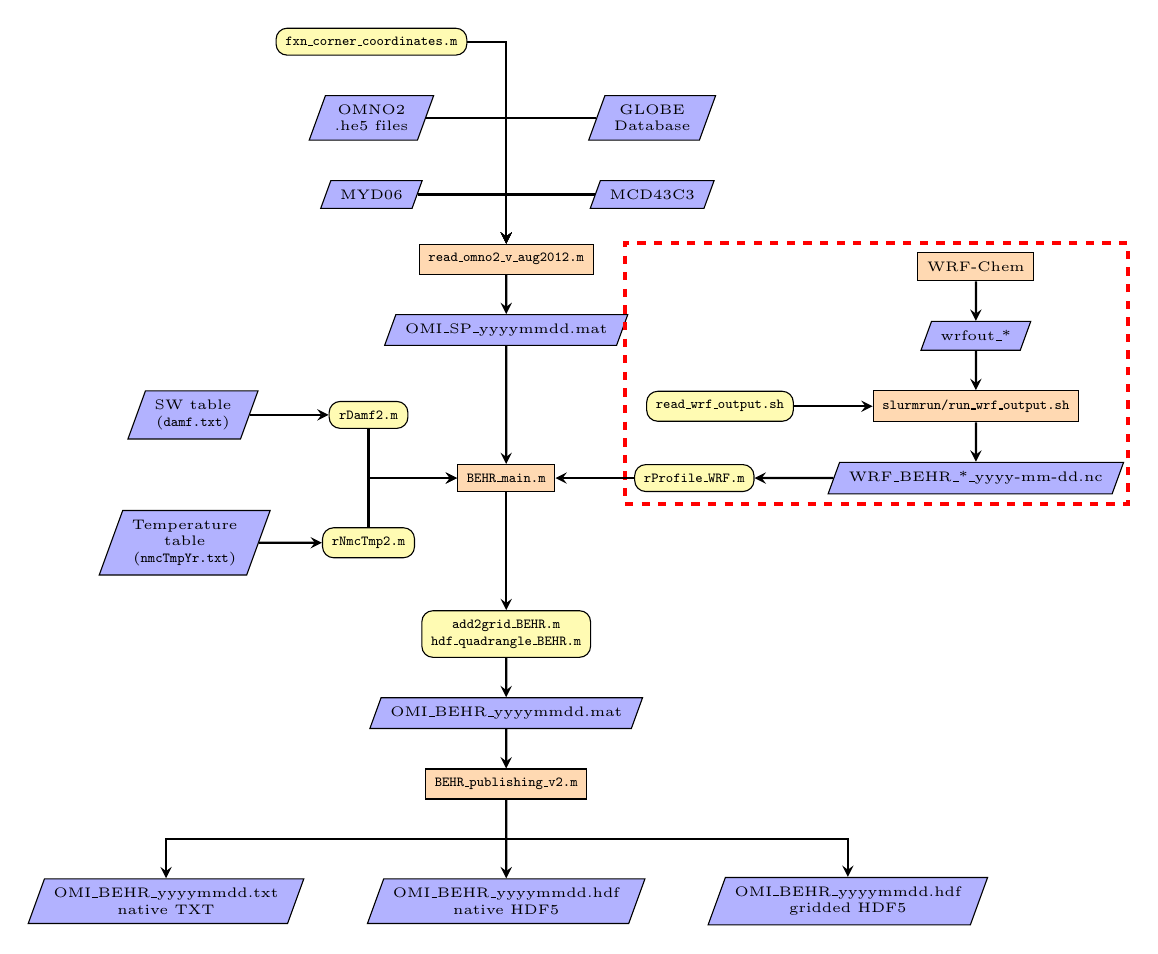
\begin{tikzpicture}[node distance=0.5cm and 1cm,every text node part/.style={align=center}]
	\node (omno2) [io] {OMNO2 \\ .he5 files};
	\node (modcld) [io, below=of omno2] {MYD06};
	\node (space1) [spacer, right=of modcld] {};
	\node (modalb) [io, right=of space1] {MCD43C3};
	\node (globe) [io, above=of modalb] {GLOBE \\ Database};
	\node (corners) [subprocess, above=of omno2] {\texttt{fxn\_corner\_coordinates.m}};
	\node (read) [process, below=of space1] {\texttt{read\_omno2\_v\_aug2012.m}};
	
	\node (omisp) [io, below=of read] {OMI\_SP\_yyyymmdd.mat};
	\node (behrmain) [process, below=of omisp, yshift=-1cm] {\texttt{BEHR\_main.m}};
	\node (space2) [spacer, left=of behrmain] {};
	\node (rDamf2) [subprocess, above=of space2] {\texttt{rDamf2.m}};
	\node (rNmcTmp2) [subprocess, below=of space2] {\texttt{rNmcTmp2.m}};
	\node (swtab) [io, left=of rDamf2] {SW table \\ (\texttt{damf.txt})};
	\node (temptab) [io, left=of rNmcTmp2, xshift=0.2cm] {Temperature \\ table \\ (\texttt{nmcTmpYr.txt})};
	\node (rProfileWRF) [subprocess, right=of behrmain] {\texttt{rProfile\_WRF.m}};
	\node (profiles) [io, right=of rProfileWRF] {WRF\_BEHR\_*\_yyyy-mm-dd.nc};
	\node (runwrf) [process, above=of profiles] {\texttt{slurmrun/run\_wrf\_output.sh}};
	\node (readwrf) [subprocess, left=of runwrf] {\texttt{read\_wrf\_output.sh}};
	\node (wrfout) [io, above=of runwrf] {wrfout\_*};
	\node (wrfchem) [process, above=of wrfout] {WRF-Chem};
		
	\node (grid) [subprocess, below=of behrmain,yshift=-1cm] {\texttt{add2grid\_BEHR.m} \\ \texttt{hdf\_quadrangle\_BEHR.m}};
	\node (omibehr) [io, below=of grid] {OMI\_BEHR\_yyyymmdd.mat};
	
	\node (publish) [process, below=of omibehr] {\texttt{BEHR\_publishing\_v2.m}};
	\node (space3) [coordinate, below=of publish] {};
	\node (behrhdf) [io, below=of space3] {OMI\_BEHR\_yyyymmdd.hdf \\ native HDF5};
	\node (behrtxt) [io, left=of behrhdf] {OMI\_BEHR\_yyyymmdd.txt \\ native TXT};
	\node (behrgridded) [io, right=of behrhdf] {OMI\_BEHR\_yyyymmdd.hdf \\ gridded HDF5};
	
	\node (development) [draw=red, line width=1.5pt, dashed, fit=(rProfileWRF) (profiles) (runwrf) (readwrf) (wrfout) (wrfchem)] {};
	
	\draw [arrow] (omno2) -| (read);
	\draw [arrow] (modcld) -| (read);
	\draw [arrow] (modalb) -| (read);
	\draw [arrow] (globe) -| (read);
	\draw [arrow] (corners) -| (read);
	
	\draw [arrow] (read) -- (omisp);
	\draw [arrow] (omisp) -- (behrmain);
	
	\draw [arrow] (swtab) -- (rDamf2);
	\draw [arrow] (rDamf2) |- (behrmain);
	\draw [arrow] (temptab) -- (rNmcTmp2);
	\draw [arrow] (rNmcTmp2) |- (behrmain);
	\draw [arrow] (rProfileWRF) -- (behrmain);
	\draw [arrow] (profiles) -- (rProfileWRF);
	\draw [arrow] (runwrf) -- (profiles);
	\draw [arrow] (readwrf) -- (runwrf);
	\draw [arrow] (wrfout) -- (runwrf);
	\draw [arrow] (wrfchem) -- (wrfout);
	
	\draw [arrow] (behrmain) -- (grid);
	\draw [arrow] (grid) -- (omibehr);
	\draw [arrow] (omibehr) -- (publish);
	
	\draw [arrow] (publish) -- (behrhdf);
	\draw [arrow] (space3) -| (behrtxt);
	\draw [arrow] (space3) -| (behrgridded);
	
	\end{tikzpicture}
	\caption{The changes necessary to allow the use of daily \emph{a priori} profiles, marked by the red box.}
	\label{fig:dev-pgrm-flow}
	\end{figure}

	The new pieces of code are \lstinline$rProfile_WRF.m$, which replaces \lstinline$rProfile_US.m$ and reads profiles from the \lstinline$WRF_BEHR_*_yyyy-mm-dd.nc$ netCDF files instead of the .mat files used previously.  These netCDF files are produced by the Bash shell script \lstinline$slurmrun_wrf_output.sh$ or \lstinline$run_wrf_output.sh$. Ideally the difference between these two is that \lstinline$run_wrf_output.sh$ is meant to run in serial, while \lstinline$slurmrun_wrf_output.sh$ runs in parallel, using the \lstinline$srun$ command with the SLURM scheduler. However, development of \lstinline$slurmrun_wrf_output.sh$ tends to proceed more rapidly, so it is preferred although it can only be run on the Savio cluster or another cluster using the SLURM scheduler.
	
	Both scripts use the NCO tools. These are installed on the Savio cluster (although as a module that needs to be loaded) and can be installed on your computer if desired. Essentially, \lstinline$slurmrun_wrf_output.sh$ determines how to average the WRF output (monthly, daily, hourly), which set of variables to put in the final files, and whether it is preparing \emph{a priori} for OMI or TEMPO (the TEMPO one is a notional implementation at current, making certain assumptions about the operation of TEMPO). It identifies the files necessary and instantiates multiple instances of the appropriate \lstinline$read_wrf_output.sh$ (may also be \lstinline$read_wrf_tempo.sh$ or \lstinline$read_wrf_emis.sh$) to allow parallel execution.  These in turn make use of built-in NCO functions and several NCO scripts I've written to both extract the key variables and calculate several additional quantities not automatically included in the WRF output. Cutting down the files in this manner substantially reduces the amount of data that needs to be moved from a cluster capable of running WRF-Chem to whatever computer is running BEHR.
	
	This information is extracted from the raw WRF-Chem output files, \lstinline[breaklines=true]$wrfout_d0X_yyyy-mm-dd_hh:mm:ss$. My scripts assume that there is one output ``frame'' per file, that is, each file represents a single slice in time. It is possible that WRF-Chem might save multiple time slices to each file, although the resulting files will likely be huge. 
	
	\lstinline$rProfile_WRF.m$ is also fairly intelligent about how it reads and applies the \ce{NO2} profiles, accounting for different spatial resolutions as well as being able to use different temporal resolutions. However to do the latter, it expects the profiles to be organized in subfolders named by the temporal resolution of the \emph{a priori} profiles in them: ``hourly,'' ``daily,'' or ``monthly.''
	
	

\newpage
\appendix
\appendixpage
\addappheadtotoc
	
\section{Changelog}

	A notation of (dev) after the version number indicates that the full archive of BEHR data was never produced using that version (i.e. ``development only'').

\bgroup
\def\arraystretch{1.5}
	\begin{table}[h]
		\begin{longtabu} to \textwidth{| l | l | X |} \hline
			Date 		& 	Version Number		&	Description \endhead \hline
			2012		&	2.0A				&	Original version by A. Russell, using OMI SP 2 with MODIS cloud and albedo, GLOBE terrain database, and WRF-Chem profiles (12 km for full US). \\ \hline
			May 2013	&	2.0B	 (dev)		&	Version (unvalidated at this point) updated by J. Laughner to use OMI SP 2 and MODIS cloud collection 6.  Albedo, terrain products, and WRF-Chem profiles unchanged.  MODIS and GLOBE data import now done directly by \texttt{read\_omno2\_v\_aug2012}, ``preprocessing'' of these files into Matlab .mat files no longer necessary. \\ \hline
		\end{longtabu}
	\end{table}
\egroup

\section{Running downloads in the background}

\section{Setup for automatic downloads} \label{app:autodl}


\end{document}